\documentclass[8pt]{article}
\usepackage{amsmath,amssymb,amsthm}
\usepackage{xcolor} % For custom colors
\usepackage{listings}
\usepackage{hyperref}
\usepackage{geometry}
\usepackage{graphicx}
\usepackage{float}

\lstset{
    language=Python, % Change this for different languages
    basicstyle=\ttfamily\footnotesize,
    keywordstyle=\color{blue}\bfseries,
    commentstyle=\color{gray},
    stringstyle=\color{red},
    frame=single, % Adds a border around the code block
    numbers=left, % Line numbers on the left
    numberstyle=\tiny\color{gray},
    backgroundcolor=\color{lightgray!10}, % Light gray background
    tabsize=4,
    breaklines=true, % Wrap long lines
    captionpos=b, % Caption below
    showspaces=false,
    showstringspaces=false
}

\geometry{letterpaper, margin=1in}

\title{Robot Path Planning in a Warehouse}
\author{Idriss Mortadi \& Abdellah Oumida}
\date{\today}

\begin{document}
\maketitle

\section{Introduction}
In modern warehouses, autonomous robots play a crucial role in streamlining logistics by transporting goods efficiently. However, as the number of robots increases, ensuring smooth and collision-free navigation becomes a significant challenge. Poor path planning can lead to congestion, delays, and inefficient warehouse operations, negatively impacting productivity and throughput.

The problem of multi-robot path planning (MRPP) involves computing efficient routes for multiple robots navigating a shared environment while avoiding obstacles and preventing collisions. This task is particularly challenging in warehouse settings, where robots must operate in tight spaces with dynamically changing conditions. Efficient solutions must balance computational feasibility with optimality, ensuring all robots reach their destinations in minimal time while adhering to movement constraints.

To address this, we formulate the multi-robot path planning problem as a Satisfiability (SAT) problem, leveraging the efficiency of modern SAT solvers to compute collision-free paths. By encoding robot movements, obstacle constraints, and avoidance rules into Boolean variables and logical formulas, we can transform path planning into a constraint satisfaction problem solvable using SAT-solving techniques.

\section{Problem Formulation}

\subsection{Parameters}
We define the warehouse as a \emph{two-dimensional grid} of size $n \times m$, denoted as:
\[
G = \{(x,y) \mid 0 \leq x < n, \; 0 \leq y < m\}
\]
where each cell in $G$ represents a valid position in the warehouse.

\subsection{Robots}
A set of robots 
\[
R = \{r_1, r_2, \dots, r_k\}
\]
operates in the grid. Each robot $r$ has:
\begin{itemize}
    \item A \textbf{start position} $(x_{\text{start}_r}, y_{\text{start}_r})$
    \item A \textbf{goal position} $(x_{\text{goal}_r}, y_{\text{goal}_r})$
\end{itemize}

\subsection{Time Horizon}
We introduce a fixed maximum time $T$, representing the upper bound on the number of time steps a robot can take to reach its goal. The problem is then solved over a discrete sequence of time steps $t \in \{0, 1, \dots, T\}$.

\subsection{Variables}
To model the problem as a SAT instance, we define the following Boolean variables:
\begin{itemize}
    \item $P(r, x, y, t)$: \textbf{True} if robot $r$ is at position $(x, y)$ at time $t$.
    \item $O(x, y)$: \textbf{True} if there is an obstacle at position $(x,y)$.
\end{itemize}

\subsection{Constraints}
\subsubsection{Robot Can Only Be at One Cell At a Time}
This constraint ensures that each robot occupies only a single cell at any given time step.
\[
\forall r \in R,\;\forall t \in \{0,\dots,T\},\;\forall x,y \in G,\;\forall x',y' \in G; (x,y)\neq(x',y'):\quad P(r,x,y,t) \implies \neg P(r,x',y',t)
\]

\subsubsection{Movement Restricted to Free Cells}
Robots can only move to cells that are not obstacles.
\[
\forall x,y \in G,\; \forall r \in R,\; \forall t \in [0,T]:\quad O(x,y) \implies \neg P(r,x,y,t)
\]

\subsubsection{Movement to Adjacent Cells Only}
Robots can only move to adjacent cells or remain stationary at each time step.
\[
\forall r \in R,\; \forall x,y,t:\quad P(r,x,y,t) \implies \bigvee_{(\Delta x, \Delta y) \in M} P\Bigl(r,\text{clamp}(x+\Delta x,0,n-1),\text{clamp}(y+\Delta y,0,m-1),\text{clamp}(t+1,0,T)\Bigr)
\]
\begin{itemize}
    \item The function \texttt{clamp(x, 0, n)} restricts the value of \texttt{x} within the inclusive range from $0$ to $n$. If \texttt{x} is less than $0$, the function returns $0$. If \texttt{x} is greater than $n$, the function returns $n$. Otherwise, it returns \texttt{x}.
    \item Here, 
    \[
    M = \{(0, 1), (1, 0), (0, 0), (-1, 0), (0, -1)\}
    \]
    represents valid movements (up, right, stay, left, down).
\end{itemize}

\subsubsection{Collision Avoidance}
Two robots cannot occupy the same cell at the same time.
\[
\forall r,r' \in R,\; r \neq r',\; \forall x,y,t:\quad P(r,x,y,t) \implies \neg P(r',x,y,t)
\]

\subsubsection{Position Switching Prohibition}
Two robots cannot swap positions between consecutive cell $(x,y)$ at time $t$ where robot $r$ is located.
time steps.
\[
\forall r,r' \in R,\; r \neq r',\; \forall x,y,t,\; \forall (\Delta x,\Delta y) \in M \setminus \{(0,0)\}:
\]
\[
P(r,x,y,t) \wedge P(r',x+\Delta x,y+\Delta y,t) \implies \neg \Bigl(P(r,x+\Delta x,y+\Delta y,t+1) \wedge P(r',x,y,t+1)\Bigr)
\]
\subsection{Objective}
The goal is to compute a valid set of paths for all robots such that:
\begin{itemize}
    \item All robots reach their designated goals within the time horizon $T$.
    \item All constraints are satisfied.
    \item (Optional) The total path length or time taken is minimized.
\end{itemize}


\section{Results}
\subsection{Basic Scenario}
Consider a simple warehouse scenario with three robots, as shown in Figure \ref{fig:warehouse_solution}. The blue robot starts at the top left and needs to reach the bottom right, the green robot starts at the bottom right and needs to reach the top left, and the red robot starts at the bottom left and needs to reach the top right. The time horizon is $10$.
    \begin{figure}[H]
    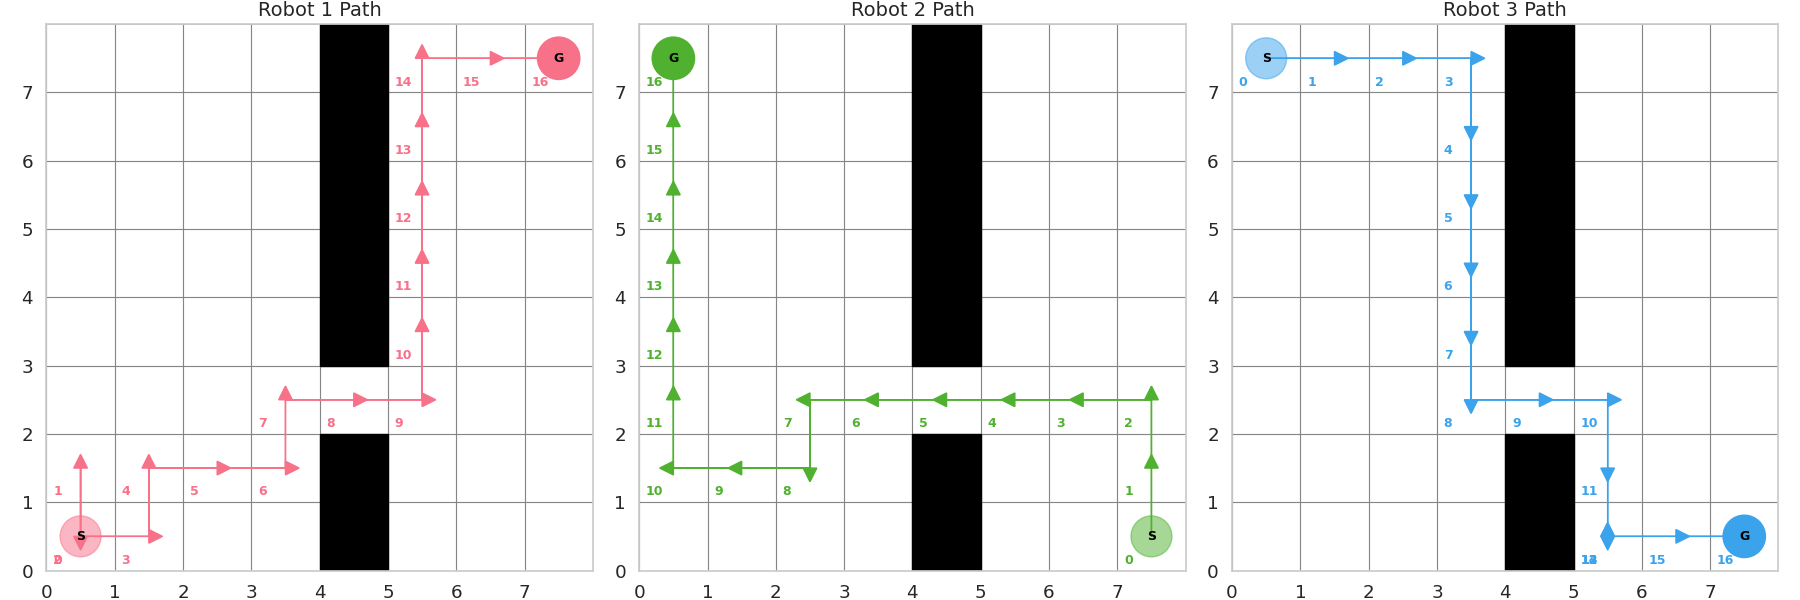
\includegraphics[width=\textwidth]{figures/warehouse_solution.png}
    \caption{A solution for a simple warehouse scenario with three robots. The blue robot starts at the top left and needs to reach the bottom right, the green robot starts at the bottom right and needs to reach the top left, and the red robot starts at the bottom left and needs to reach the top right. The time horizon is 10.}
    \label{fig:warehouse_solution}
\end{figure}


\section{Implementation Details}

\subsection{Classes and Data Structures}

\subsubsection*{Position}
\begin{itemize}
    \item \textbf{Attributes:} 
    \begin{itemize}
        \item \texttt{x}: Integer representing the x-coordinate.
        \item \texttt{y}: Integer representing the y-coordinate.
    \end{itemize}
    \item \textbf{Methods:}
    \begin{itemize}
        \item \texttt{\_hash\_}: Returns a hash value based on the coordinates.
        \item \texttt{\_eq\_}: Checks equality between two \texttt{Position} instances.
    \end{itemize}
\end{itemize}

\subsubsection*{Robot}
\begin{itemize}
    \item \textbf{Attributes:}
    \begin{itemize}
        \item \texttt{id}: Unique identifier for the robot.
        \item \texttt{start}: \texttt{Position} object representing the starting position.
        \item \texttt{goal}: \texttt{Position} object representing the goal position.
    \end{itemize}
\end{itemize}

\subsection{WarehousePathPlanner Class}
\emph{Attributes:}
\begin{itemize}
    \item \texttt{width}: Width of the warehouse grid.
    \item \texttt{height}: Height of the warehouse grid.
    \item \texttt{time\_horizon}: Maximum time steps allowed.
    \item \texttt{cnf}: CNF formula to store constraints.
    \item \texttt{var\_map}: Mapping of variable names to integers.
    \item \texttt{next\_var}: Next available variable number.
    \item \texttt{moves}: List of valid movements (stay, up, right, down, left).
\end{itemize}

\emph{Methods:}
\begin{itemize}
    \item \texttt{create\_variable(robot\_id, x, y, t)}: Creates a variable representing a robot's position at a given time.
    \item \texttt{add\_initial\_positions(robots)}: Adds constraints for the initial positions of robots.
    \item \texttt{add\_goal\_positions(robots)}: Adds constraints for the goal positions of robots.
    \item \texttt{add\_obstacle\_constraints(obstacles, robots)}: Adds constraints to prevent robots from occupying obstacle positions.
    \item \texttt{add\_movement\_constraints(robots)}: Adds constraints for valid movements between time steps.
    \item \texttt{add\_collision\_avoidance(robots)}: Adds constraints to prevent robots from occupying the same position.
    \item \texttt{add\_position\_switching\_prohibition(robots)}: Adds constraints to prevent robots from switching positions.
    \item \texttt{add\_implication(antecedent, consequents)}: Adds implication constraints to the CNF formula.
    \item \texttt{solve()}: Solves the SAT problem and returns the solution if one exists.
    \item \texttt{decode\_solution(solution)}: Converts the SAT solution to robot paths.
\end{itemize}

\subsection{Code Commentary}

\subsubsection*{Imports and Data Structures}

\begin{lstlisting}
import itertools
from dataclasses import dataclass
from typing import Dict, List, Optional, Set

from pysat.formula import CNF
from pysat.solvers import Glucose3
\end{lstlisting}

\textbf{Interpretation:}
\begin{itemize}
    \item \texttt{itertools}: Provides functions for efficient looping, useful for generating combinations.
    \item \texttt{dataclasses}: Simplifies the creation of classes that primarily store data.
    \item \texttt{typing}: Provides support for type hints, enhancing code readability and maintainability.
    \item \texttt{pysat.formula} and \texttt{pysat.solvers}: Used for creating and solving SAT problems.
\end{itemize}

\subsubsection*{Position Class}

\begin{lstlisting}
@dataclass(frozen=True)
class Position:
    x: int
    y: int

    def _hash_(self):
        return hash((self.x, self.y))

    def _eq_(self, other):
        if not isinstance(other, Position):
            return NotImplemented
        return self.x == other.x and self.y == other.y
\end{lstlisting}

\textbf{Interpretation:}
\begin{itemize}
    \item Represents a position in the grid with \texttt{x} and \texttt{y} coordinates.
    \item \texttt{frozen=True} makes instances immutable and hashable, allowing them to be used as keys in dictionaries.
    \item \texttt{\_hash\_} and \texttt{\_eq\_} enable comparison and hashing of \texttt{Position} objects.
\end{itemize}

\subsubsection*{Robot Class}

\begin{lstlisting}
@dataclass
class Robot:
    id: int
    start: Position
    goal: Position
\end{lstlisting}

\textbf{Interpretation:}
\begin{itemize}
    \item Represents a robot with a unique \texttt{id}, a starting \texttt{Position}, and a goal \texttt{Position}.
\end{itemize}

\subsection{WarehousePathPlanner Class Overview}
The \texttt{WarehousePathPlanner} class encapsulates the logic for modeling the multi-robot path planning problem as a SAT instance. Key aspects include:

\subsubsection*{Initialization}
\begin{lstlisting}
def __init__(self, width: int, height: int, time_horizon: int):
    self.width = width
    self.height = height
    self.time_horizon = time_horizon
    self.cnf = CNF()
    self.var_map = {}
    self.next_var = 1
    # Valid movements: stay in place, move up, right, down, or left.
    self.moves = [(0, 0), (0, 1), (1, 0), (0, -1), (-1, 0)]
\end{lstlisting}

\textbf{Interpretation:}
\begin{itemize}
    \item The planner is aware of the grid dimensions and the available time steps.
    \item The CNF object and variable mappings are initialized for building the SAT instance.
    \item The allowed movements include staying in place along with directional changes.
\end{itemize}

\subsubsection*{Creating Variables}
\begin{lstlisting}
def create_variable(self, robot_id: int, x: int, y: int, t: int) -> int:
    key = f"R{robot_id}X{x}Y{y}T{t}"
    if key not in self.var_map:
        self.var_map[key] = self.next_var
        self.next_var += 1
    return self.var_map[key]
\end{lstlisting}

\textbf{Interpretation:}
\begin{itemize}
    \item Generates a unique variable for each robot, position, and time configuration.
    \item The descriptive key (e.g., \texttt{"R1X2Y3T4"}) supports traceability in the SAT variables.
\end{itemize}

\subsubsection*{Adding Initial Position Constraints}
\begin{lstlisting}
def add_initial_positions(self, robots: List[Robot]):
    for robot in robots:
        start_var = self.create_variable(robot.id, robot.start.x, robot.start.y, 0)
        self.cnf.append([start_var])
        for x in range(self.width):
            for y in range(self.height):
                var = self.create_variable(robot.id, x, y, 0)
                if x != robot.start.x or y != robot.start.y:
                    self.cnf.append([-var])
\end{lstlisting}

\textbf{Interpretation:}
\begin{itemize}
    \item The robot is fixed at its starting position at time $0$ via a positive clause.
    \item All other cells at time $0$ are negated, enforcing that the robot can only start at its designated location.
\end{itemize}

\subsubsection*{Adding Goal Position Constraints}
\begin{lstlisting}
def add_goal_positions(self, robots: List[Robot]):
    for robot in robots:
        goal_var = self.create_variable(robot.id, robot.goal.x, robot.goal.y, self.time_horizon)
        self.cnf.append([goal_var])
        for x in range(self.width):
            for y in range(self.height):
                if x != robot.goal.x or y != robot.goal.y:
                    var = self.create_variable(robot.id, x, y, self.time_horizon)
                    self.cnf.append([-var])
\end{lstlisting}

\textbf{Interpretation:}
\begin{itemize}
    \item Ensures each robot is at its designated goal at the final time step.
    \item Prohibits the robot from being in any other cell at time $T$.
\end{itemize}

\subsubsection*{Adding Obstacle Constraints}
\begin{lstlisting}
def add_obstacle_constraints(self, obstacles: Set[Position], robots: List[Robot]):
    for obstacle in obstacles:
        if not (0 <= obstacle.x < self.width and 0 <= obstacle.y < self.height):
            raise ValueError("Obstacle is outside the warehouse bounds")
        for robot in robots:
            for t in range(self.time_horizon + 1):
                var = self.create_variable(robot.id, obstacle.x, obstacle.y, t)
                self.cnf.append([-var])
\end{lstlisting}

\textbf{Interpretation:}
\begin{itemize}
    \item Prevents any robot from occupying cells designated as obstacles at any time step.
\end{itemize}

\subsubsection*{Adding Movement Constraints}
\begin{lstlisting}
def add_movement_constraints(self, robots: List[Robot]):
    for robot in robots:
        for t in range(self.time_horizon + 1):
            positions_at_t = []
            for x in range(self.width):
                for y in range(self.height):
                    var = self.create_variable(robot.id, x, y, t)
                    positions_at_t.append(var)
            self.cnf.append(positions_at_t)
            for pos1, pos2 in itertools.combinations(positions_at_t, 2):
                self.cnf.append([-pos1, -pos2])
            if t < self.time_horizon:
                for x in range(self.width):
                    for y in range(self.height):
                        current_pos = self.create_variable(robot.id, x, y, t)
                        next_positions = []
                        for dx, dy in self.moves:
                            next_x, next_y = x + dx, y + dy
                            if 0 <= next_x < self.width and 0 <= next_y < self.height:
                                next_pos = self.create_variable(robot.id, next_x, next_y, t + 1)
                                next_positions.append(next_pos)
                        if next_positions:
                            self.add_implication(current_pos, next_positions)
\end{lstlisting}

\textbf{Interpretation:}
\begin{itemize}
    \item Ensures that at every time step a robot occupies exactly one cell.
    \item Enforces that if a robot is at a given position at time $t$, then it moves to one of the valid positions at time $t+1$.
\end{itemize}

\newpage
\subsubsection*{Adding Collision Avoidance Constraints}
\begin{lstlisting}
def add_collision_avoidance(self, robots: List[Robot]):
    for t in range(self.time_horizon + 1):
        for x in range(self.width):
            for y in range(self.height):
                robot_vars = []
                for robot in robots:
                    var = self.create_variable(robot.id, x, y, t)
                    robot_vars.append(var)
                for var1, var2 in itertools.combinations(robot_vars, 2):
                    self.cnf.append([-var1, -var2])
\end{lstlisting}

\textbf{Interpretation:}
\begin{itemize}
    \item Prevents more than one robot from occupying the same cell at the same time.
\end{itemize}

\subsubsection*{Adding Position Switching Prohibition}
\begin{lstlisting}
def add_position_switching_prohibition(self, robots: List[Robot]):
    for t in range(self.time_horizon):
        for x1 in range(self.width):
            for y1 in range(self.height):
                for dx, dy in self.moves[1:]:
                    x2, y2 = x1 + dx, y1 + dy
                    if 0 <= x2 < self.width and 0 <= y2 < self.height:
                        for r1, r2 in itertools.combinations(robots, 2):
                            r1_pos1_t = self.create_variable(r1.id, x1, y1, t)
                            r2_pos2_t = self.create_variable(r2.id, x2, y2, t)
                            r1_pos2_t1 = self.create_variable(r1.id, x2, y2, t + 1)
                            r2_pos1_t1 = self.create_variable(r2.id, x1, y1, t + 1)
                            self.cnf.append([-r1_pos1_t, -r2_pos2_t, -r1_pos2_t1, -r2_pos1_t1])
\end{lstlisting}

\textbf{Interpretation:}
\begin{itemize}
    \item Prevents two robots from swapping positions between consecutive time steps.
\end{itemize}

\subsubsection*{Adding Implication Constraints}
\begin{lstlisting}
def add_implication(self, antecedent: int, consequents: List[int]):
    self.cnf.append([-antecedent] + consequents)
\end{lstlisting}

\textbf{Interpretation:}
\begin{itemize}
    \item This helper function expresses the implication that if the antecedent is true, then at least one of the consequents must be true.
\end{itemize}

\subsubsection*{Solving and Decoding the SAT Problem}
\begin{lstlisting}
def solve(self) -> Optional[Dict[str, bool]]:
    with Glucose3() as solver:
        solver.append_formula(self.cnf.clauses)
        if solver.solve():
            model = solver.get_model()
            if not isinstance(model, list):
                raise ValueError("No model found")
            return {
                var_name: lit > 0
                for var_name, var_num in self.var_map.items()
                for lit in model
                if abs(lit) == var_num
            }
        return None
\end{lstlisting}

\begin{lstlisting}
def decode_solution(self, solution: Dict[str, bool]) -> Dict[int, List[Position]]:
    paths = {}
    for var_name, is_true in solution.items():
        if is_true:
            numbers = "".join(c if c.isdigit() else " " for c in var_name).split()
            robot_id, x, y, t = map(int, numbers)
            if robot_id not in paths:
                paths[robot_id] = [None] * (self.time_horizon + 1)
            paths[robot_id][t] = Position(x, y)
    for path in paths.values():
        if None in path:
            raise ValueError("Invalid solution: incomplete path detected")
    return paths
\end{lstlisting}

\textbf{Interpretation:}
\begin{itemize}
    \item The \texttt{solve} function uses the Glucose3 solver to obtain a satisfying assignment.
    \item The \texttt{decode\_solution} function reconstructs robot paths from the model, ensuring each time step is accounted for.
\end{itemize}

\subsubsection*{Decoding the SAT Solution}
\begin{lstlisting}
def decode_solution(self, solution: Dict[str, bool]) -> Dict[int, List[Position]]:
    paths = {}
    for var_name, is_true in solution.items():
        if is_true:
            numbers = "".join(c if c.isdigit() else " " for c in var_name).split()
            robot_id, x, y, t = map(int, numbers)
            if robot_id not in paths:
                paths[robot_id] = [None] * (self.time_horizon + 1)
            paths[robot_id][t] = Position(x, y)
    for path in paths.values():
        if None in path:
            raise ValueError("Invalid solution: incomplete path detected")
    return paths
\end{lstlisting}

\textbf{Interpretation:}  
\begin{itemize}
    \item \emph{Solution Decoding:} This method parses each true SAT variable (e.g., \texttt{"R1X2Y3T4"} corresponds to robot 1 being at position $(2,3)$ at time 4) from the solution.
    \item \emph{Reconstructing Paths:} It reconstructs the complete path for each robot over the entire time horizon.
    \item \emph{Completeness Check:} The method ensures that every time step contains a valid position. If any time step is missing, it raises an error indicating an incomplete path.
\end{itemize}

\end{document}